\subsection{Impact of lattice calculations of  $x$-space PDFs}
\label{sec:projectionsxspace}

In the previous section, we studied the impact of
lattice-QCD calculations of PDF moments, and we now
perform an initial exploration of the
potential constraints that future lattice QCD calculations
of $x$-space PDFs can provide on global analyses.
%
We focus on the isotriplet
combination $x u-x d$ (and $x\Delta u - x\Delta d$
in the polarised case),  
which is the quark combination that has been the focus of initial
studies. It is simpler to calculate, owing to the lack of disconnected
diagrams and the absence of mixing with other quark flavours or with
gluons.


Following the same Bayesian reweighting procedure employed for PDF moments
in Sect.~\ref{sec:projections:rw},
we have generated pseudo-data for the isotriplet
combinations
\be
\label{eq:isotriplet_unpol}
u(x_i,Q^2)-d(x_i,Q^2) \, \quad{\rm and} \, \quad
\bar{u}(x_i,Q^2)-\bar{d}(x_i,Q^2) \, , \quad i=1,\ldots,N_x \, ,
\ee
for the unpolarised case, and for
\be
\label{eq:isotriplet_pol}
\Delta u(x_i,Q^2)-\Delta d(x_i,Q^2) \, \quad{\rm and} \, \quad
\Delta\bar{u}(x_i,Q^2)-\Delta\bar{d}(x_i,Q^2) \, , \quad i=1,\ldots,N_x \, ,
\ee
for the polarised case, with $N_x$ being the number of points
in $x$-space that are being sampled and we
take $Q^2=4$ GeV$^2$, consistent with our choices for the PDF moment exercise.

We consider here three scenarios, denoted by scenario D, E, and F,
for the total uncertainty $\delta_L$
that will be assigned to
the lattice-QCD calculations of the specific quark
combinations listed in Eqns.~(\ref{eq:isotriplet_unpol})
and~(\ref{eq:isotriplet_pol}).
%
%First of all we indicate the values of $\left\{ x_i \right\}$
%that have been chosen for this exercise.
%
Lattice-QCD computations are expected to have the smallest systematic 
uncertainties at large $x$, so we choose the $N_x=5$ points to be
\be
x_i = 0.70\, ,0.75,\, 0.80,\, 0.85, \, 0.90 \, .
\ee
Then, for each scenario, we assume the same relative error for each value of 
$\{x_i\}$, and, moreover, we neglect possible correlations between 
neighbouring $x$-points.
%
We assume uncertainties of $\delta_{L}=12\%, 6\%$ and 3\% for scenarios
D, E, and F, respectively.
%
Note that we assume the same values of $\delta_{L}$ for the polarised
and unpolarised cases, as well as for both the quark
and the antiquark isotriplet combinations Eqns.~(\ref{eq:isotriplet_unpol})
and~(\ref{eq:isotriplet_pol}).

We summarise the results of this exercise in Fig.~\ref{fig:impactxspace}, 
where we plot the ratio of the PDF uncertainties in each scenario A, B and C 
(D, E and F) to the uncertainty of the original
NNPDF3.1 (NNPDFpol1.1) data set.
%
We show the impact on the PDF uncertainties
in $\bar{u}$ and $\bar{d}$ at large-$x$ in the upper
plots, with the corresponding comparison for $\Delta\bar{u}$
and $\Delta\bar{d}$ in the lower plots.
%
From this comparison, we find that lattice-QCD calculations of the 
$x$-dependence of PDFs can significantly reduce the uncertainties for both 
unpolarised and polarised antiquarks in the large-$x$ region.
%
Taking into account that the PDF uncertainties on the large-$x$
antiquarks are rather large, and that they
enter a number of important BSM search channels
(such as for instance for new heavy gauge bosons $W'$ and $Z'$),
our analysis demonstrates that such calculations would have direct
phenomenological implications.
%
In a Monte Carlo approach such as NNPDF, the
PDF uncertainties themselves fluctuate, particularly at low-scales,
explaining the wiggles in these plots.

%-------------------------------------------------------------------
\begin{figure}[!t]
\centering
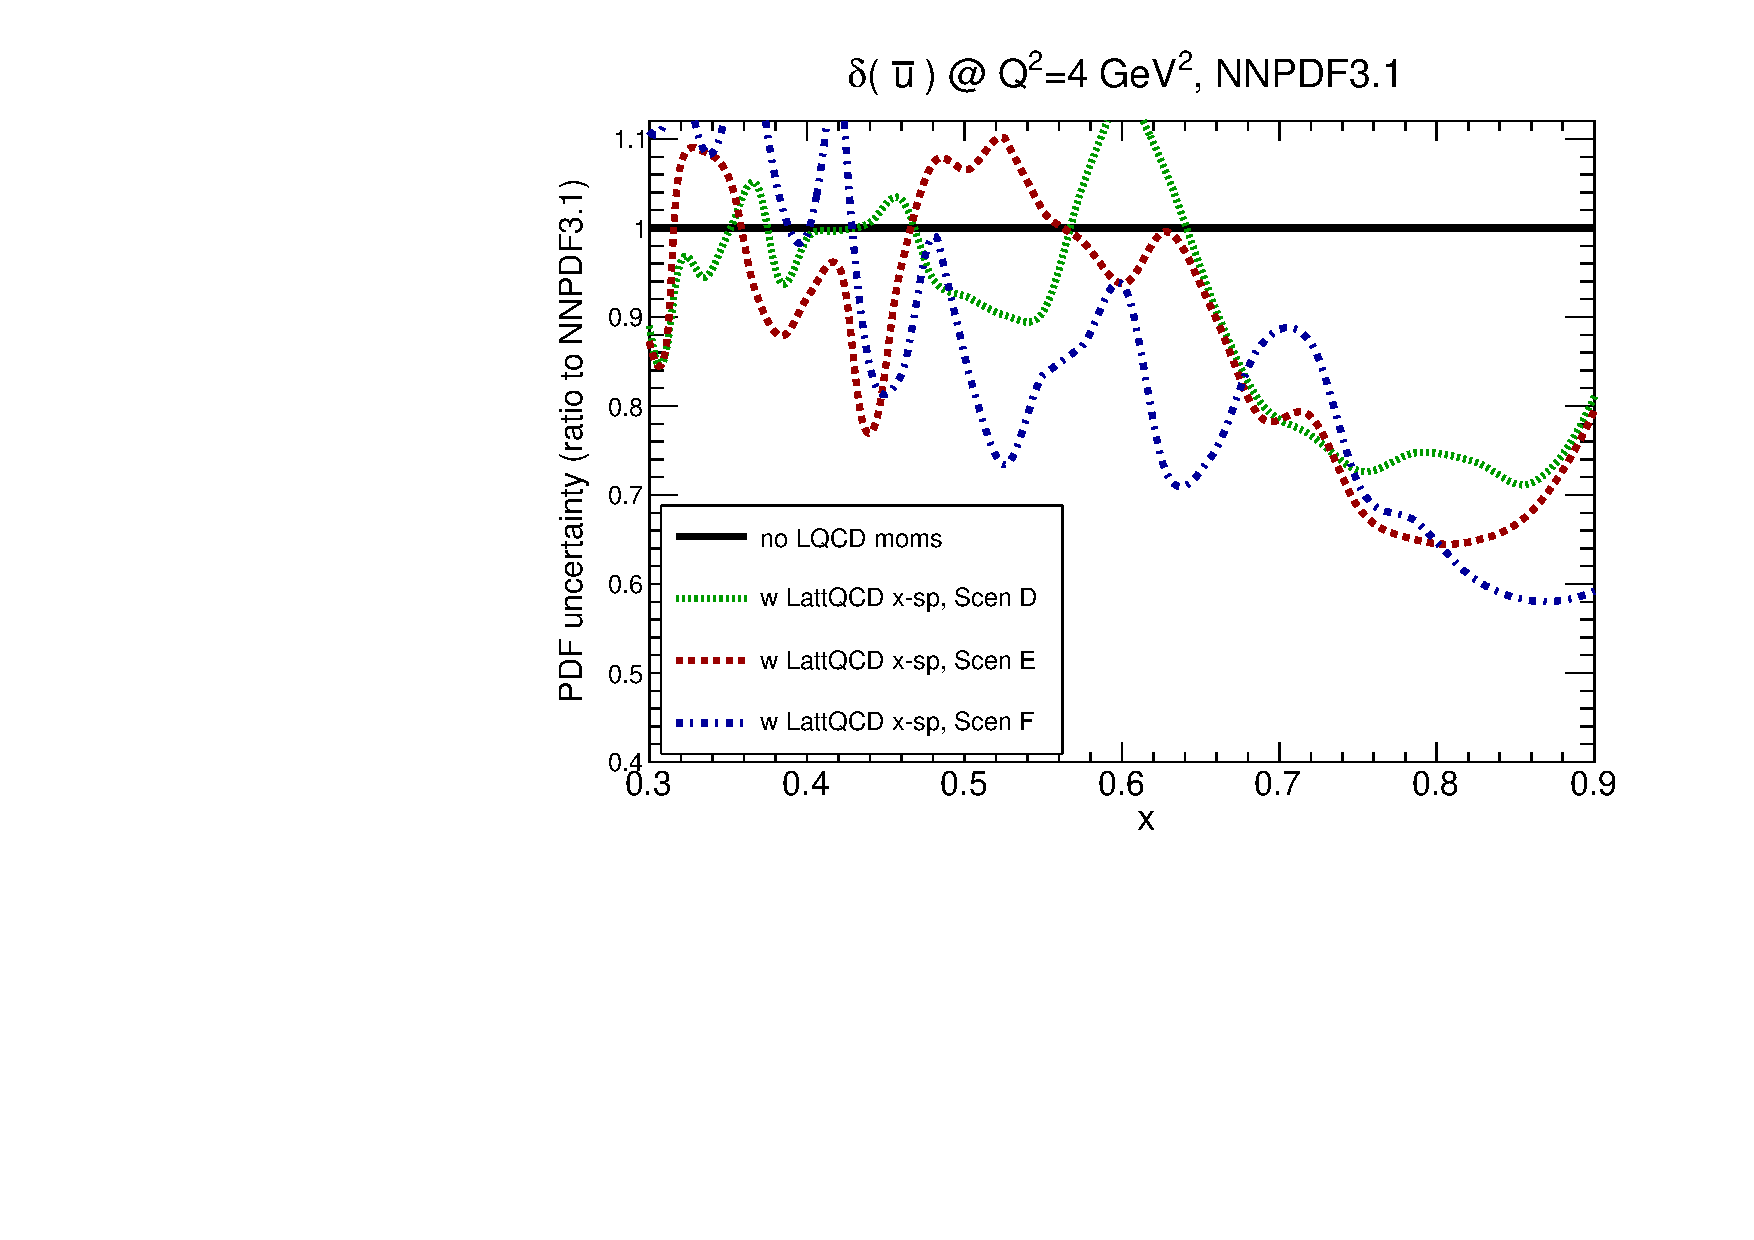
\includegraphics[scale=0.45]{plots/xubar-unpol-lattice-relerr-xdata-xspace.pdf}
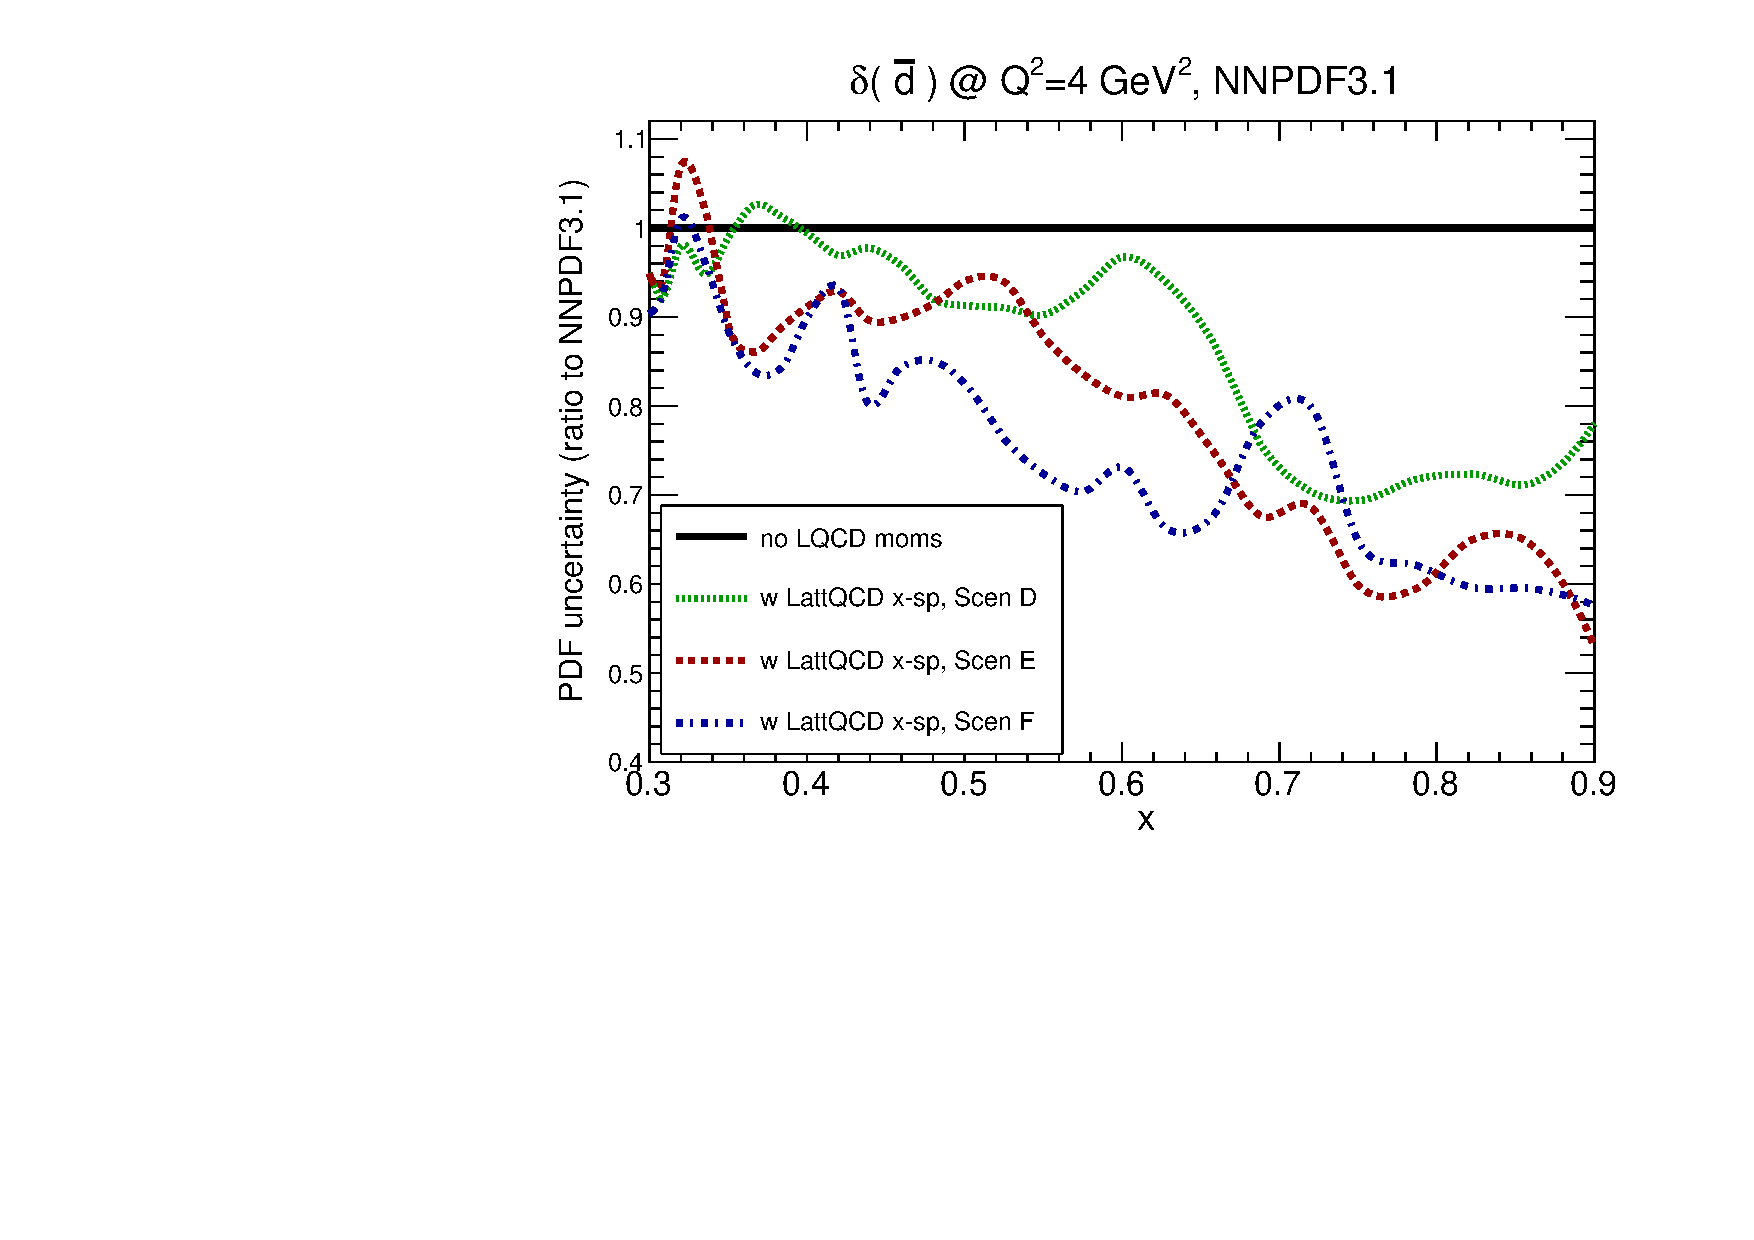
\includegraphics[scale=0.45]{plots/xdbar-unpol-lattice-relerr-xdata-xspace.pdf}
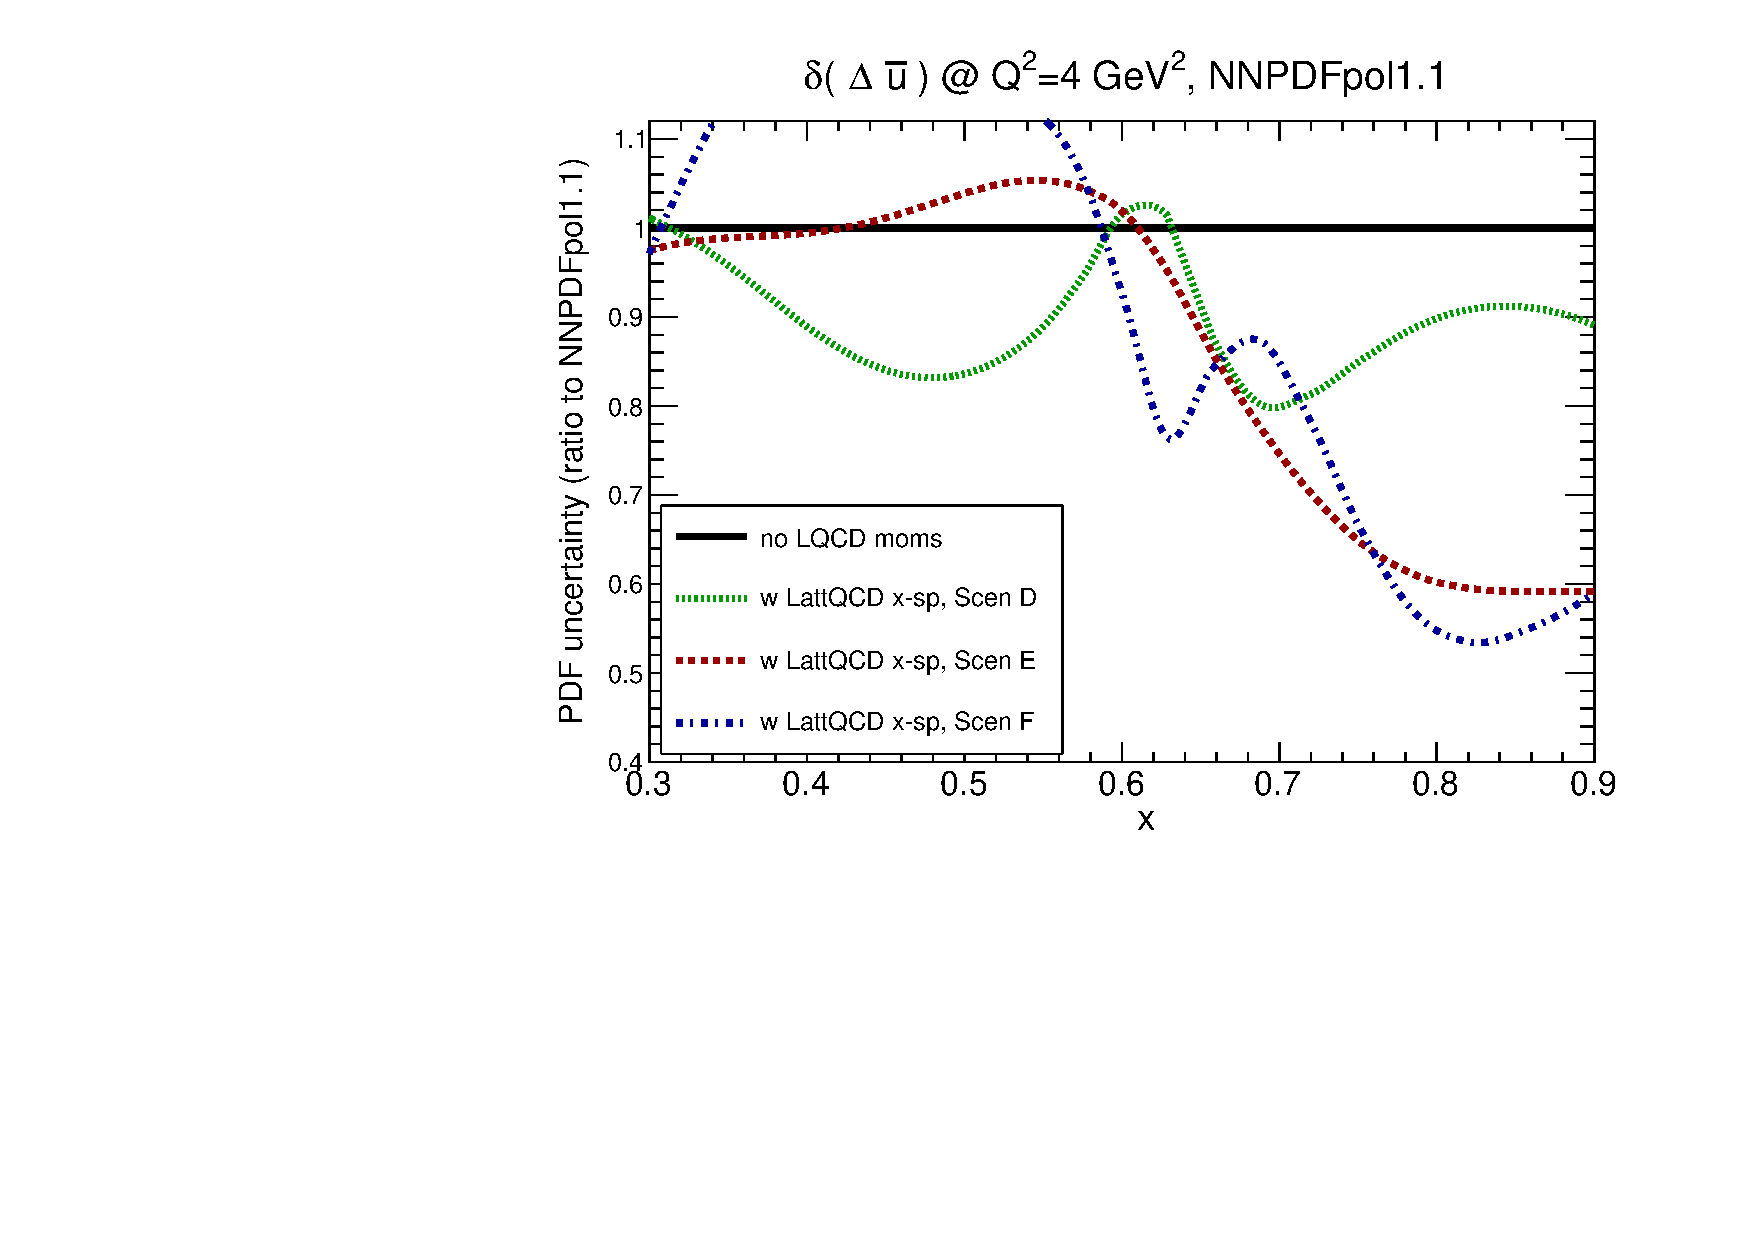
\includegraphics[scale=0.45]{plots/xubar-pol-lattice-relerr-xdata-xspace.pdf}
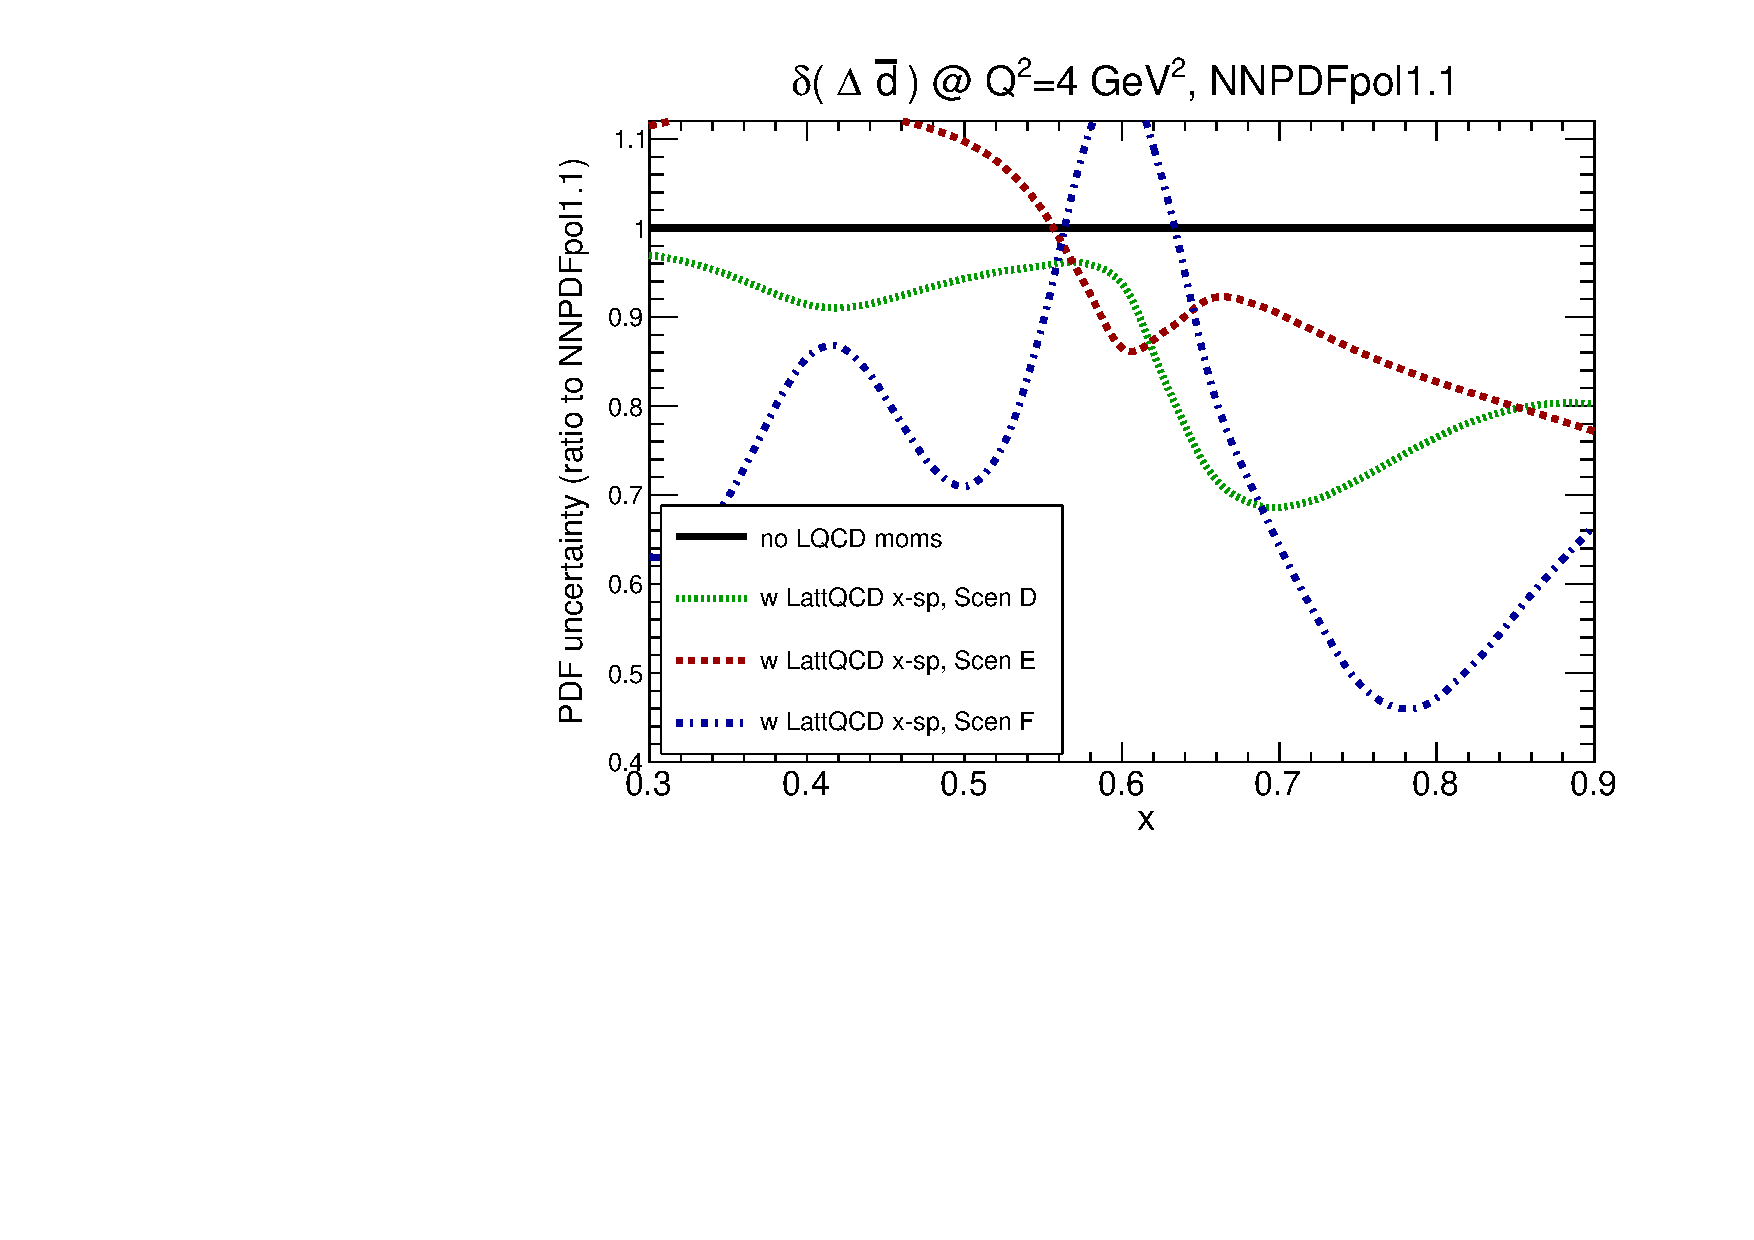
\includegraphics[scale=0.45]{plots/xdbar-pol-lattice-relerr-xdata-xspace.pdf}
\caption{\small The ratio of PDF uncertainties to the original
  NNPDF3.1 (NNPDFpol1.1) in the fits where lattice-QCD pseudo-data
  on $x$-space PDFs has been added to the global unpolarised
  (polarised) analysis.
  %
  Specifically, we show the impact on the PDF uncertainties
  in $\bar{u}$ and $\bar{d}$ at large-$x$ in the upper
  plots, with the corresponding comparison for $\Delta\bar{u}$
  and $\Delta\bar{d}$ in the lower plots.
}    
\label{fig:impactxspace}
\end{figure}
%---------------------------------------------------------------------

Fig.~\ref{fig:impactxspace} shows that
in the unpolarised case the large-$x$ PDF uncertainties could be reduced
to $60\%$ of their original value.
%
We also find that there are no large
differences between the three
scenarios, suggesting that a direct lattice-QCD calculation
of $x \bar{u}-x \bar{d}$ does not need to reach uncertainties
at the few-percent level to influence global fits.
%
For the polarised PDFs, Fig.~\ref{fig:impactxspace} demonstrates that the
reduction in PDF uncertainties could be significantly more marked.
%
For instance, in the case of $\Delta \bar{d}$, at $x\simeq 0.8$
the resulting PDF uncertainty from scenario F is less than 50\%
of the original uncertainty.

In Tab.~\ref{tab:neffxspace} we indicate the effective number of replicas
$N_{\rm eff}$, Eq.~(\ref{eq:effnrep}), remaining when
the lattice-QCD pseudo-data for Eqns.~(\ref{eq:isotriplet_unpol})
and~(\ref{eq:isotriplet_pol}) are included in the global
   unpolarised and polarised fits.
   %
   Here we find a marked decrease in $N_{\rm rep}$
   for the three scenarios,
   in particular for the unpolarised case.
   %
   For example, in the most optimistic scenario F, only
   64 effective replicas remain out of the
   original sample of $N_{\rm rep}=1000$ replicas.
   %
   See Tab.~\ref{tab:neff} for the corresponding
   information at the level of PDF moments.
   
%%%%%%%%%%%%%%%%%%%%%%%%%%%%%%%%%%%%%%%%%%%%%%
\begin{table}[h!]
  \centering
  \renewcommand{\arraystretch}{1.3} 
  \begin{tabular}{c|c|c}
    \hline
    &  NNPDF3.1  &  NNPDFpol1.1 \\
    \hline
    \hline
    $N_{\rm rep}$ original   &   1000 &  100   \\
    \hline
     $N_{\rm eff}$ Scenario D    &   376  &  41   \\
     $N_{\rm eff}$ Scenario E    &   173   &   35  \\
     $N_{\rm eff}$ Scenario F   &   64  &   22  \\
    \hline
  \end{tabular}
  \caption{\small The effective number of replicas
    $N_{\rm eff}$, Eq.~(\ref{eq:effnrep}), remaining when the pseudo-data
    on the lattice-QCD calculations
    of Eqns.~(\ref{eq:isotriplet_unpol})
and~(\ref{eq:isotriplet_pol}) 
   are included in the global
    unpolarised and polarised fits. 
    \label{tab:neffxspace}
  }
\end{table}
%%%%%%%%%%%%%%%%%%%%%%%%%%%%%%%%%%%%%%%%%%%%%%

We emphasise that
the results of this exercise have to be interpreted
with some care.
%
First of all, the results depend sensitively on the specific values of
$\left\{ x_i \right\}$
that we have assumed for the lattice-QCD calculation,
and on the values
of the associated uncertainties $\delta_L$.
%
The quantitative results depend on the choice of input PDF set and would 
vary if, for example, the input set was the HERAPDF2.0 set used for the 
Hessian profiling exercise of Sect.~\ref{sec:hessianprofiling}.
%
Even with these caveats, our analysis makes clear that a direct
computation of the isotriplet combination $x u-x d$ on the lattice
has the potential to constrain the large-$x$ PDFs in
a more significant way than corresponding PDF moment calculations,
particularly in the unpolarised case.
%
Given the importance of antiquark PDFs in the large-$x$ region for LHC phenomenology,
pursuing these calculations should be high on the list
of priorities for the lattice-QCD community.

%%%%%%%%%%%%%%%%%%%%%%%%%%%%%%%%%%%%%%%%%%%%%%%%%
